\documentclass[a4paper,14pt]{article}

\usepackage{comment} % Para comentar várias linhas ao mesmo tempo

%matemática
\usepackage{amsmath}
\usepackage{amssymb}

%diagramação
\usepackage{extsizes}
\everymath{\displaystyle}
\usepackage{geometry}
\usepackage{fancyhdr}
\usepackage{multicol}
\usepackage{graphicx}
\usepackage[brazil]{babel}
\usepackage[shortlabels]{enumitem}
\usepackage{cancel}
\usepackage{textcomp}
\usepackage{tcolorbox}

%tabelas
\usepackage{array} % Para melhor formatação de tabelas
\usepackage{longtable}
\usepackage{booktabs}  % Para linhas horizontais mais bonitas
\usepackage{float}   % Para usar o modificador [H]
\usepackage{caption} % Para usar legendas em tabelas
\usepackage{wrapfig} % Para usar tabelas e figuras flutuantes
\usepackage{xcolor} % Para cores do fundo de tabelas
\usepackage{colortbl} % Para cores do fundo de tabelas

%tikzpicture
\begin{comment}
	\usepackage{tikz}
	\usepackage{scalerel}
	\usepackage{pict2e}
	\usepackage{tkz-euclide}
	\usetikzlibrary{calc}
	\usetikzlibrary{patterns,arrows.meta}
	\usetikzlibrary{shadows}
	\usetikzlibrary{external}
\end{comment}


%pgfplots
\usepackage{pgfplots}
\pgfplotsset{compat=newest}
\usepgfplotslibrary{statistics}
\usepgfplotslibrary{fillbetween}

%colours
\usepackage{xcolor}



\columnsep=2cm
\hoffset=0cm
\textwidth=8cm
\setlength{\columnseprule}{.1pt}
\setlength{\columnsep}{2cm}
\renewcommand{\headrulewidth}{0pt}
\geometry{top=1in, bottom=1in, left=0.7in, right=0.5in}

\pagestyle{fancy}
\fancyhf{}
\fancyfoot[C]{\thepage}

\begin{document}
	
	\noindent\textbf{6FMA141 - Matemática} 
	
	\begin{center}Conjunto dos múltiplos e mmc (Versão estudante)
	\end{center}
	
	\noindent\textbf{Nome:} \underline{\hspace{10cm}}
	\noindent\textbf{Data:} \underline{\hspace{4cm}}
	
	%\section*{Questões de Matemática}
	
	\begin{multicols}{2}
	    \noindent Para $a \in \mathbb{Z}$, temos que o conjunto de seus múltiplos será: \\
	    $M(a) = \{x \in \mathbb{Z}: a | x\}$ \\
	    Para $a, b, c \in \mathbb{Z}^*$, temos:
	    \begin{itemize}
	    	\item mmc $(a, b)$ = mín. $(M_+^*(a) \cap M_+^*(b))$
	    	\item mmc $(a, b)$ = mmc $(b, a)$ = mmc $(|a|, |b|)$
	    	\item mmc $(a, b, c)$ = mmc (mmc $(a, b), c$) 
	    \end{itemize}
		\noindent\textsubscript{--------------------------------------------------------------------------}
		\begin{enumerate} 
			\item Apresentar:
			\begin{enumerate}[a)]
				\item $M(3)$ \\\\\\\\\\\\\\\\
				\item $M(-3)$ \\\\\\\\\\\\\\\\
				\item $M_+^*(1)$ \\\\\\\\\\\\\\\\
				\item 6\{1, -1, 3, -3\} \\\\\\\\\\\\\\\\
				\item 2\{0, 3, 6\} \\\\\\\\\\\\\\\\
			\end{enumerate}
			\item Calcular, usando a definição, o mmc de:
			\begin{enumerate}[a)]
				\item 2 e 5. \\\\\\\\\\\\\\\\
				\item -4 e 8. \\\\\\\\\\\\\\\\
				\item 3 e 4. \\\\\\\\\\\\\\\\
				\item 6 e -24. \\\\\\\\\\\\\\\\
				\item 1 e 7. \\\\\\\\\\\\\\\\
			\end{enumerate}
			\item Refaça o exercício anterior usando o diagrama de Venn. \newpage
			\item Calcular, usando a definição, o mmc de:
			\begin{enumerate}[a)]
				\item 2, 4 e 6. \\\\\\\\\\\\\\\\
				\item -1, 1, 2 e 4. \\\\\\\\\\\\\\\\
			\end{enumerate}
			\textbf{Desafio olímpico} \\\\
			(OBMEP) As contas $AB \cdot C = 195$ e $CDE : F = 88$ estão corretas, sendo $A, B, C, D, E$ e $F$ algarismos diferentes. O número $AB$ é formado pelos algarismos $A$ e $B$, e o número $CDE$ é formado pelos algarismos $C, D$ e $E$. Qual é o algarismo representado pela letra $F$? \\
			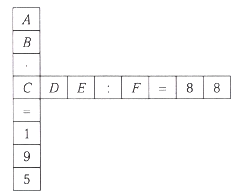
\includegraphics[width=1\linewidth]{6FMA141_imagens/imagem1}
			\begin{enumerate}[a)]
				\item 1
				\item 2
				\item 4
				\item 6
				\item 8
			\end{enumerate}
			%70 a 73
			\item Calcular, usando a definição, o mmc de:
			\begin{enumerate}[a)]
				\item 8 e 12.
				\item 16 e 40.
				\item -4 e 18.
				\item -3, 6 e -12.
			\end{enumerate}
			\item Determine:
			\begin{enumerate}[a)]
				\item 2 números cujo mmc seja 20.
				\item 2 números cujo mmc seja 48.
			\end{enumerate}
			\item Determine:
			\begin{enumerate}[a)]
				\item $M(3)$ \\\\\\\\\\\\\\
				\item $M_+(9)$ \\\\\\\\\\ 
				\item $5\mathbb{N}$ \\\\\\\\\\
				\item $8\mathbb{Z}_+^*$ \\\\\\\\\\
				\item 6\{3, 4, 5\} \\\\\\\\\\
				\item $4\mathbb{Z}_-$ \\\\\\\\\\
			\end{enumerate}
			\item Calcule o mmc dos números a seguir utilizando o diagrama de Venn:
			\begin{enumerate}[a)]
				\item 2 e 9 \\\\\\\\
				\item 6 e 10 \\\\\\\\\\\\\\
				\item 2 e 7 \\\\\\\\\\\\\\
			\end{enumerate}
		\end{enumerate}
		$~$ \\ $~$ \\ $~$ \\ $~$ \\ $~$ \\ $~$ \\ $~$ \\ $~$ \\ $~$ \\ $~$ \\ $~$ \\ $~$ \\ $~$ \\ $~$ \\ $~$ \\ $~$ \\ $~$ \\ $~$ \\ $~$ \\ $~$ \\ $~$ \\ $~$ \\ $~$ \\ $~$ \\ $~$
	\end{multicols}
\end{document}